

\subsection{Entanglement in a spin chain with 2 qubits}
In this section, we analyze the dynamics of a 
system consisting of two qubits with the Hamiltonian given by:

\[
    \hamil =  \hbar J\left [ \left ( \frac{1 + \delta}{2} \right ) \sigma_1^x \otimes 
    \sigma_2^x  + \left ( \frac{1 - \delta}{2} \right ) \sigma_1^y \otimes \sigma_2^y \right ] + 
    D \hbar \left ( \sigma_1^x \otimes \sigma_2^y + \gamma \sigma_1^y \otimes \sigma_2^x  \right ) + g \left( 
    \sigma_1^z \otimes \mathbb{\hat{I}} + \mathbb{\hat{I}} \otimes \sigma_2^z  
\right).
\]

we focus on the concurrence $C(\rho(t))$, which quantifies the entanglement between 
the two qubits. The analytical solution for the concurrence, as derived in Appendix B, is given by:

\begin{equation*}
        C(\rho(t)) = \abs*{\sin(2 \mu t)},
\end{equation*}

where \(\mu = \sqrt{J^2 + D^2(\gamma-1)^2}\).

We plot the concurrence in the figure 


We can see the plot of $C(\ket{\psi (t)})$ for the $\ket{\psi (t)}$ at \myeqref{eq: psi t} in the figure 

    \begin{figure}[h!]
        \centering
        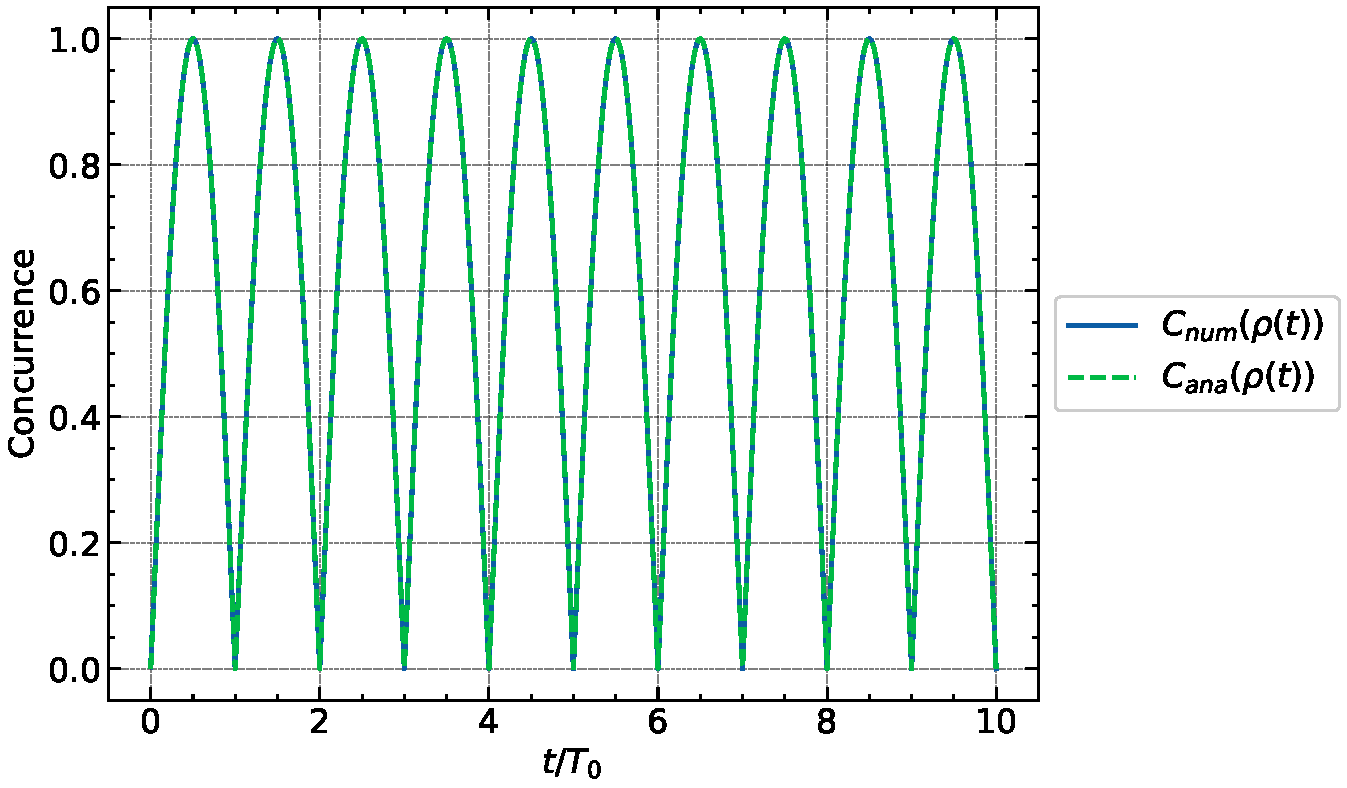
\includegraphics[width=0.8\linewidth]{results_and_discussion/2_qubits/up_down_with_ana_0.pdf}
        \caption{\centering $D=0$, Mean Squared Error: 1.51e-07, $\gamma = -1$, $\delta = 1$, $g = 1$, $J = 1$}
        \label{fig:concurrencecpsiD_0}
    \end{figure}
    \begin{figure}[h!]
        \centering
        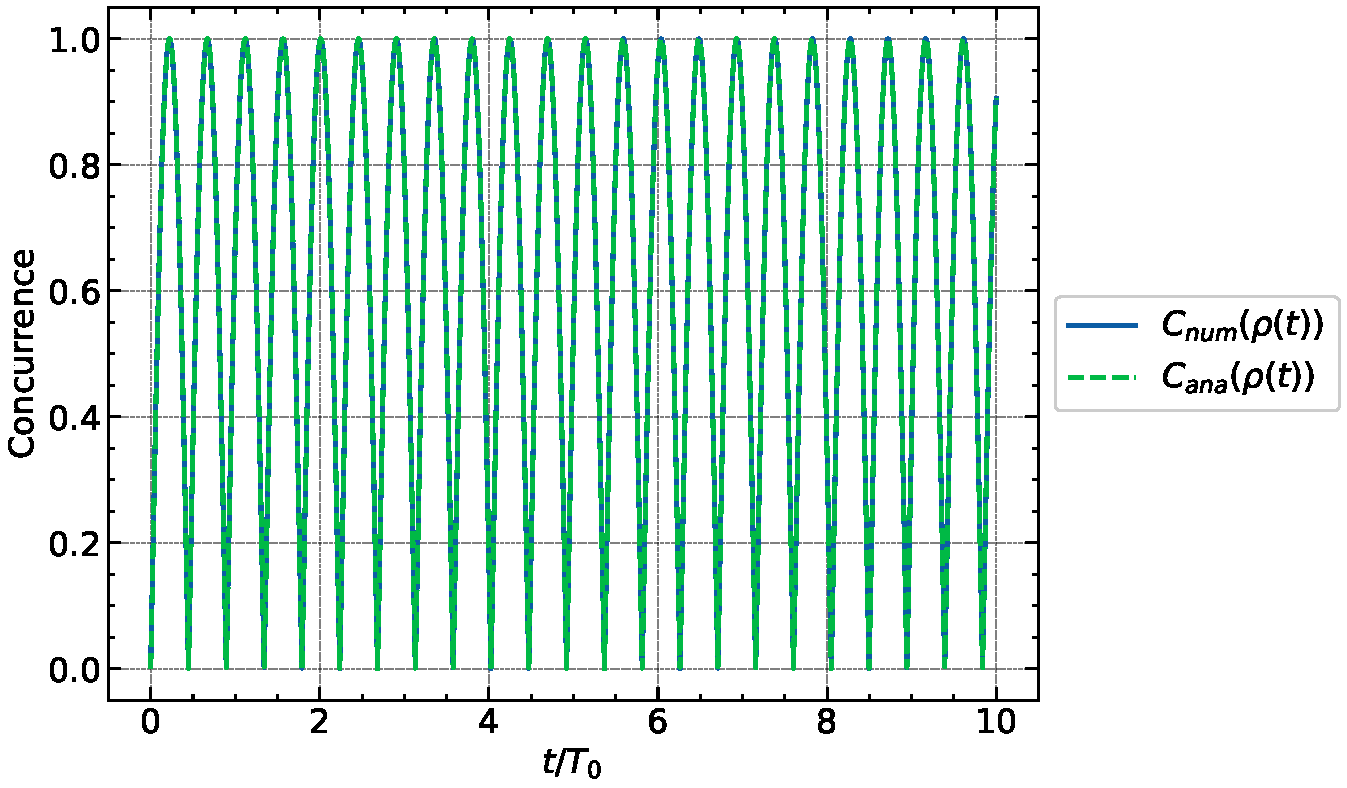
\includegraphics[width=0.8\linewidth]{results_and_discussion/2_qubits/up_down_with_ana_1.pdf}
        \caption{\centering $D=1$, Mean Squared Error: 1.51e-07, $\gamma = -1$, $\delta = 1$, $g = 1$, $J = 1$}
        \label{fig:concurrencecpsiD_1}
    \end{figure}

\newpage

The concurrence formula reveals a simple yet profound oscillatory behavior of the entanglement between the qubits. The parameter \(\mu\) plays a crucial role in determining the frequency of these oscillations, which depends on the coupling constants \(J\) and \(D\) as well as the anisotropy parameter \(\gamma\).

\textbf{Impact of Coupling Constants \(J\) and \(D\):}

The coupling constant \(J\) directly contributes to \(\mu\), indicating that a stronger XX and YY interaction 
        leads to faster oscillations in concurrence. The term \(D(\gamma-1)\) suggests 
        that the effect of the \(D\) coupling on the concurrence 
        is modulated by the anisotropy \(\gamma\). For \(\gamma = 1\), 
        this contribution vanishes, and the oscillation frequency is 
        solely determined by \(J\). However, for \(\gamma \neq 1\), 
        the anisotropy introduces additional dynamics through \(D\).


 \textbf{Behavior for Different Regimes of \(\mu\):}

 When \(\mu\) is large (e.g., large \(J\) 
        or significant anisotropy), the concurrence oscillates 
        rapidly, meaning that the system frequently transitions 
        between entangled and separable states. For small \(\mu\), the oscillations are slower, 
        indicating more prolonged periods of either high or low entanglement.

\textbf{Maximal Concurrence:}
 The concurrence achieves its maximum value of 1 when \(\sin(2 \mu t) = \pm 1\), indicating a fully entangled state.
 Conversely, \(C(\ket*{\psi(t)}) = 0\) when \(\sin(2 \mu t) = 0\), representing separable states where the qubits are not entangled.

\subsection{Discussion}

The results provide significant insights into the entanglement 
dynamics in a two-qubit system with anisotropic and cross-coupling terms. 
The oscillatory nature of the concurrence reflects the intricate interplay 
between different types of interactions present in the Hamiltonian. 
This behavior is essential for applications in quantum information 
processing, where control over entanglement is crucial.

\begin{itemize}
    \item \textbf{Quantum Control:} By tuning the parameters 
    \(J\), \(D\), and \(\gamma\), one can manipulate 
    the entanglement dynamics, potentially allowing for 
    the design of specific quantum gates or the 
    implementation of quantum error correction protocols that rely on dynamic entanglement.

    \item \textbf{Effect of Anisotropy:} The dependence of \(\mu\) on 
    \(\gamma\) illustrates how anisotropy can either enhance or diminish 
    the contribution of the \(D\) coupling to the entanglement dynamics. 
    This result suggests that systems with tunable anisotropy could be 
    particularly versatile in quantum control schemes.

    \item \textbf{Robustness of Entanglement:} The periodic nature of the concurrence indicates that, under specific conditions, entanglement can be robust over time, recurring predictably as a function of time. This property might be exploited to maintain entanglement over long durations in quantum communication protocols.
\end{itemize}

In Conclusion
 concurrence 
 quantifies the entanglement between two qubits. 
 For example, when \(t/T_0 = 0.5 + k\), where \(k \in \mathbb{N}\), the concurrence is 1. At this time, the state \(\ket{\psi (t)}\) is:


 
 \begin{equation*}
 	\ket{\psi \left( t = \frac{\pi}{4} + \frac{k\pi}{2}\right) } = \frac{1}{\sqrt{2}} \ket{\uparrow \downarrow} - \frac{i(J + iD(\gamma -1))}{\sqrt{2}\gamma}   \ket{\downarrow \uparrow}
 \end{equation*}
 
 
This state is evidently entangled according to the definition.

Moreover we can recognize a Bell state we this form: 

\begin{equation}
		\ket{\psi \left( t = \frac{\pi}{4} + \frac{k\pi}{2}\right) } = \frac{1}{\sqrt{2}} \left(  \ket{\uparrow \downarrow} -ie^{i\theta}\ket{\uparrow \downarrow}  \right)
\end{equation}

where $ \theta = \arctan\left( \frac{D(\gamma -1)}{J}\right)$


 
And at $t/T_0 = k$ the concurrence equal to $0$, 

 \begin{equation*}
	\ket{\psi \left( t = \frac{k\pi}{2}\right) } = \frac{i(J + iD(\gamma -1))}{\sqrt{2}\gamma}   \ket{\downarrow \uparrow}
\end{equation*}

In this case, the state is separable.
	

\newpage
\subsection{Entanglement in a spin chain with N qubits}
This study systematically investigates the concurrence in a three-qubit system and a six-qubit system
governed by the Heisenberg XY model, incorporating the Dzyaloshinskii-Moriya interaction (DMI). 
The primary parameters analyzed include the DMI constant \(D\), the anisotropy parameter \(\delta\), and the correction factor 
\(\gamma\). The concurrence between pairs of qubits was assessed under various configurations of these parameters.


\subsubsection{Entanglement in a spin chain with 3 qubits}


The concurrence values varied from 0.0 to approximately 0.8, indicating robust entanglement within the qubit system. 
The pairwise concurrences \( (C_{1,2}, C_{1,3}, C_{2,3}) \) exhibited a consistent pattern, with entanglement gradually 
diminishing over time.

In the first subfigure \refig{fig:subfig1}, the concurrence values show a peak of approximately 0.8 with \( D = 0 \), \( \gamma = 1 \), and \( \delta = 0 \). With an increase in the anisotropy parameter to \( \delta = 1 \) \refig{fig:subfig2}, 
the concurrence values remained relatively high, albeit slightly lower than in the previous case. The maximum concurrence observed 
was around 0.6, with a similar temporal decline in entanglement distribution across the qubits.

The introduction of DMI with \( D = 1 \) \refig{fig:subfig3} resulted in a slight enhancement of concurrence values, reaching a peak of 
approximately 0.8. This suggests that DMI strengthens the entanglement between qubits, with the pairwise concurrences following a similar pattern 
to earlier configurations but with marginally higher values.

When both \( D \) and \( \delta \) were set to 1 \refig{fig:subfig4}, the concurrence values were slightly lower, 
peaking at about 0.6. The entanglement distribution remained similar across qubit pairs, 
though the overall entanglement was reduced compared to 
the scenario with \( D = 1 \) and \( \delta = 0 \).

\begin{figure}[h!]
    \centering
    \begin{subfigure}[b]{0.48\textwidth}
        \centering
        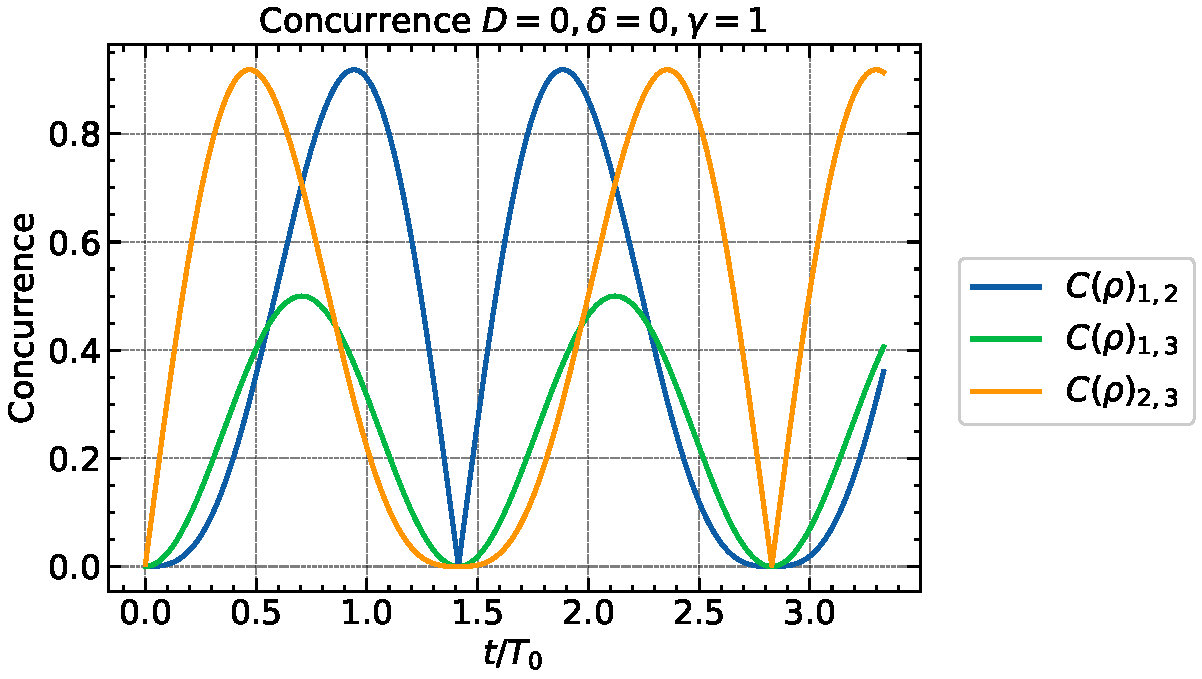
\includegraphics[width=\linewidth]{results_and_discussion/3_qubits/up_down_with_ana_0_1_0.pdf}
        \caption{Concurrence for \( D = 0\), \( \gamma = 1\), \( \delta = 0\)}
        \label{fig:subfig1}
    \end{subfigure}
    \hfill
    \begin{subfigure}[b]{0.48\textwidth}
        \centering
        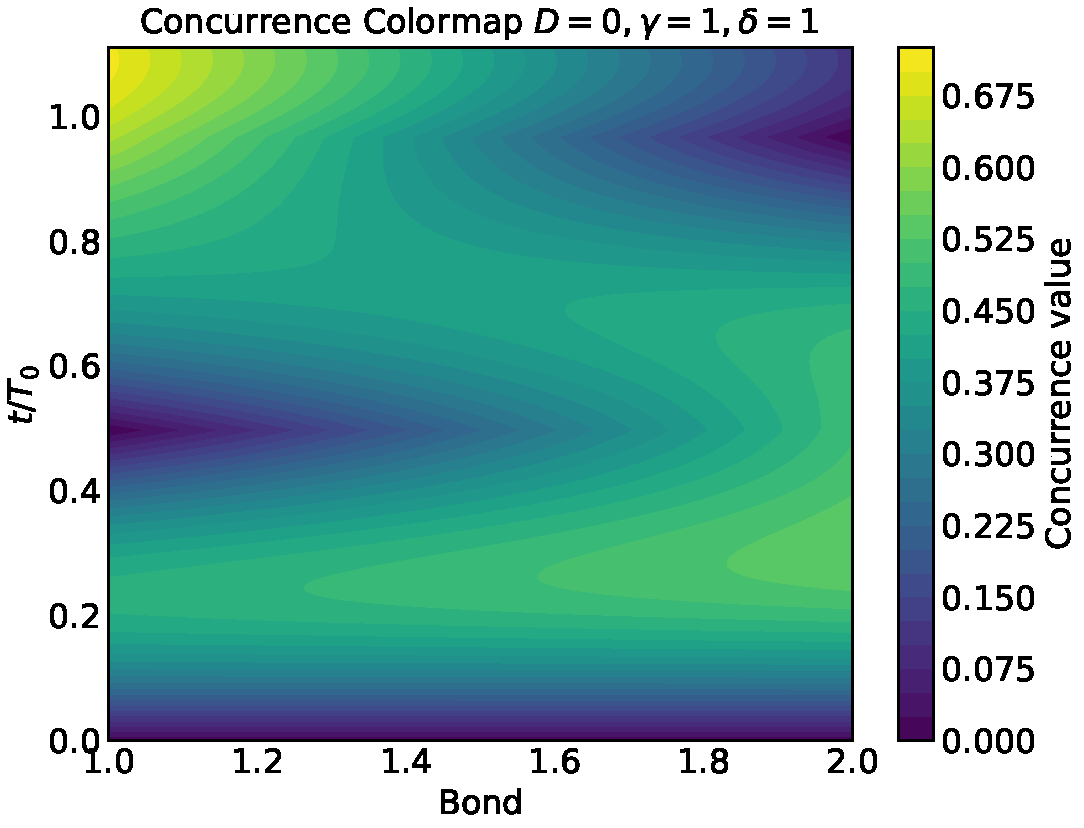
\includegraphics[width=\linewidth]{results_and_discussion/3_qubits/up_down_with_ana_0_1_1.pdf}
        \caption{Concurrence for \( D = 0\), \( \gamma = 1\), \( \delta = 1\)}
        \label{fig:subfig2}
    \end{subfigure}

    \vspace{0.5cm}

    \begin{subfigure}[b]{0.48\textwidth}
        \centering
        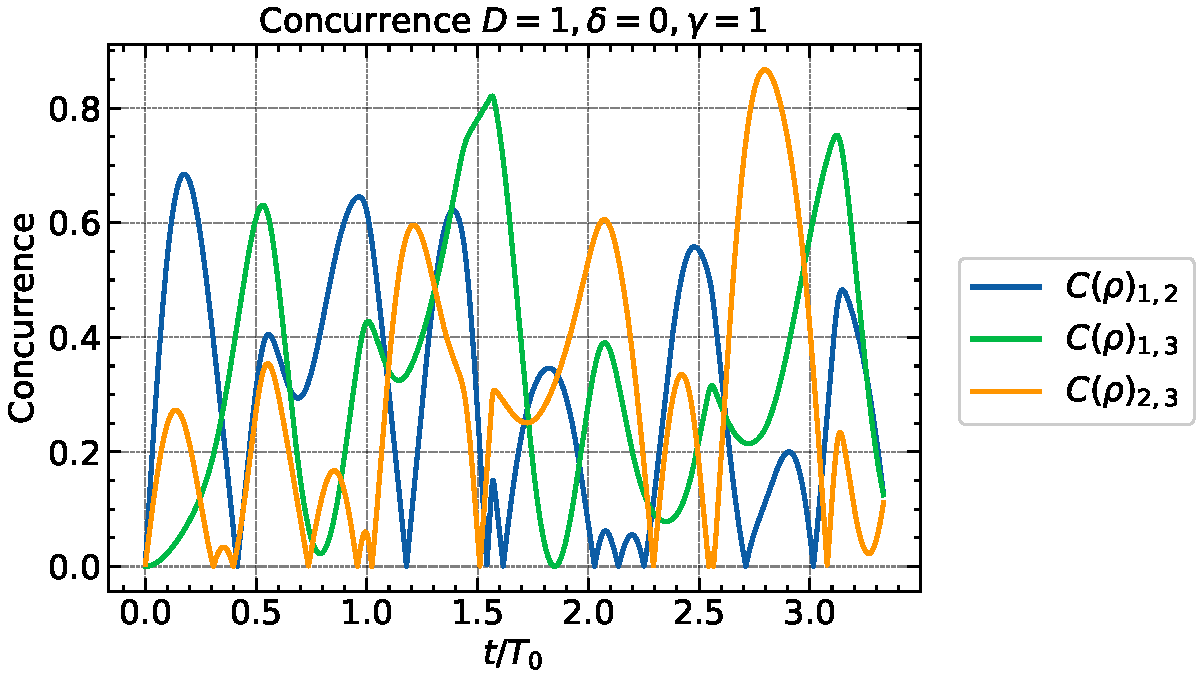
\includegraphics[width=\linewidth]{results_and_discussion/3_qubits/up_down_with_ana_1_1_0.pdf}
        \caption{Concurrence for \( D = 1\), \( \gamma = 1\), \( \delta = 0\)}
        \label{fig:subfig3}
    \end{subfigure}
    \hfill
    \begin{subfigure}[b]{0.48\textwidth}
        \centering
        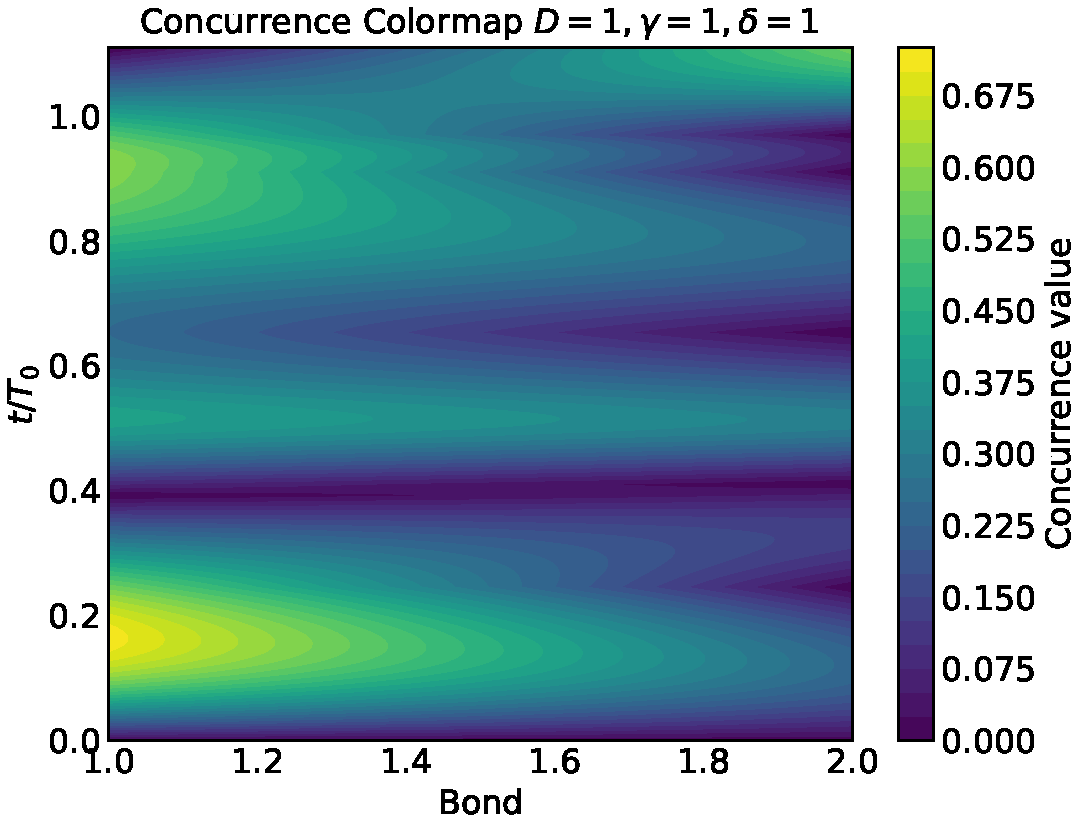
\includegraphics[width=\linewidth]{results_and_discussion/3_qubits/up_down_with_ana_1_1_1.pdf}
        \caption{Concurrence for \( D = 1\), \( \gamma = 1\), \( \delta = 1\)}
        \label{fig:subfig4}
    \end{subfigure}

    \caption{Concurrence for different values of \( D \) and \( \delta \) with \( \gamma = 1 \). The concurrence values indicate the level of entanglement in the qubit system over time, showing how different parameters influence the entanglement.}
    \label{fig:concurrence_comparison}
\end{figure}


\newpage
\textbf{Discussion}

The findings highlight the significant role of the Dzyaloshinskii-Moriya interaction in influencing the entanglement characteristics of the three-qubit system. The DMI, quantified by \(D\), generally enhances concurrence, indicating stronger entanglement. This effect is particularly pronounced when comparing scenarios with \(D = 0\) and \(D = 1\).

Conversely, the anisotropy parameter \(\delta\) introduces a competing influence that can diminish the overall entanglement as it increases. Specifically, when \(\delta = 1\), the system exhibits lower concurrence values compared to \(\delta = 0\), even in the presence of DMI. This suggests that while DMI tends to enhance entanglement, increasing \(\delta\) may counteract this effect, possibly due to modifications in the system's symmetry or interaction strengths.

In the absence of DMI (\(D = 0\)), the system still demonstrates significant entanglement, especially when \(\gamma = 1\) and \(\delta = 0\), with concurrence values reaching up to 0.8. This indicates that the Heisenberg XY model inherently supports strong entanglement, which can be modulated by adjusting the DMI and anisotropy parameters.




\newpage
\subsubsection{Entanglement in a spin chain with 6 qubits}
\textbf{Concurrence for \( D = 0, \gamma = 1, \delta = 0 \):} \refig{fig:6q_0_1_0}
The concurrence values in this configuration range from 0.00 to approximately 0.81, showing a high level of entanglement that gradually decreases as the system evolves over time. The colormap indicates a relatively uniform distribution of entanglement across the bonds in the lattice.


\textbf{Concurrence for \( D = 0, \gamma = 1, \delta = 1 \):} \refig{fig:6q_0_1_1}
When \(\delta\) is increased to 1, the maximum concurrence value decreases slightly to approximately 0.675. The distribution of concurrence values remains similar to the previous case, with the entanglement decreasing over time, but with a slightly reduced maximum entanglement value.


\textbf{Concurrence for \( D = 1, \gamma = 1, \delta = 0 \):} \refig{fig:6q_0_1_0}
Introducing the DMI constant \(D = 1\) while keeping \(\gamma = 1\) and \(\delta = 0\) leads to an increase in the maximum concurrence value to around 0.81. This increase suggests that the DMI enhances the entanglement within the system. The distribution of concurrence is still fairly uniform across the lattice, indicating that the DMI positively influences the overall entanglement.


\textbf{Concurrence for \( D = 1, \gamma = 1, \delta = 1 \):} \refig{fig:6q_1_1_1}
When both \(D\) and \(\delta\) are set to 1, the system exhibits a maximum concurrence value of approximately 0.56, 
which is lower than when \(\delta = 0\). This suggests that while the DMI increases entanglement, the anisotropy 
parameter \(\delta\) introduces an effect that reduces the overall entanglement when \(\gamma\) is also present.
\begin{figure}[h!]
    \centering
    \begin{subfigure}[b]{0.48\textwidth}
        \centering
        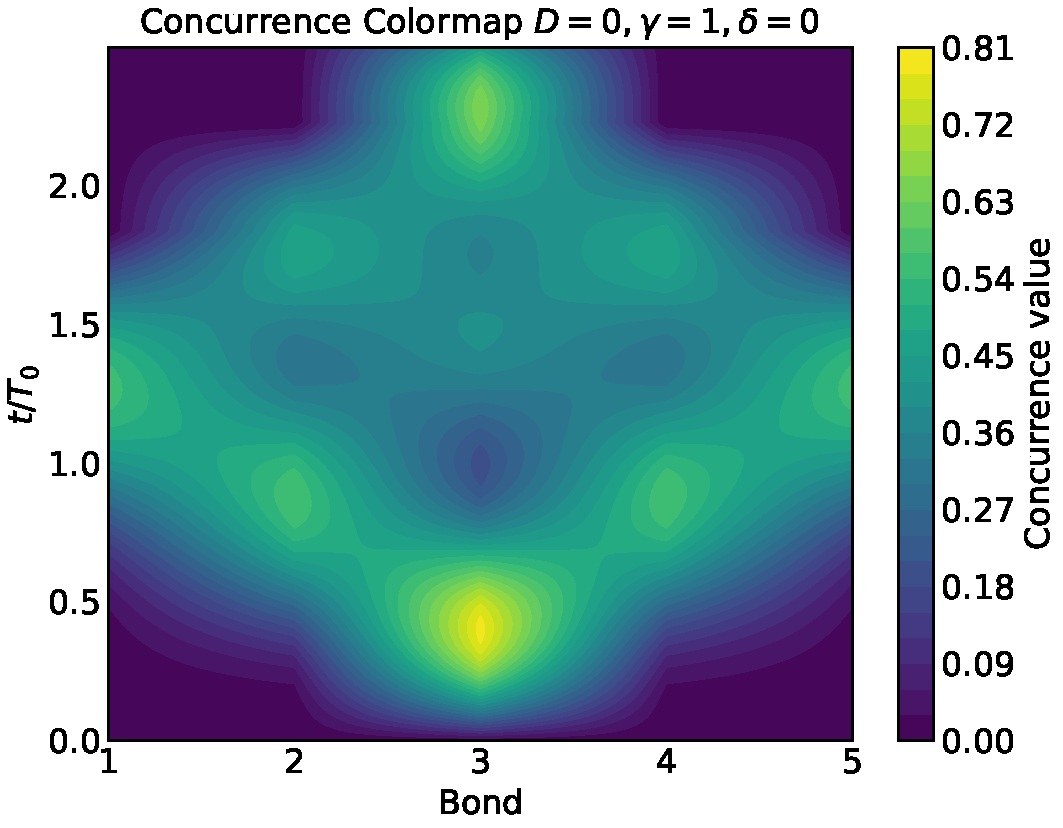
\includegraphics[width=\linewidth]{results_and_discussion/6_qubits/up_down_with_ana_0_1_0.pdf}
        \caption{Concurrence for \( D = 0, \gamma = 1, \delta = 0 \)}
        \label{fig:6q_0_1_0}
    \end{subfigure}
    \hfill
    \begin{subfigure}[b]{0.48\textwidth}
        \centering
        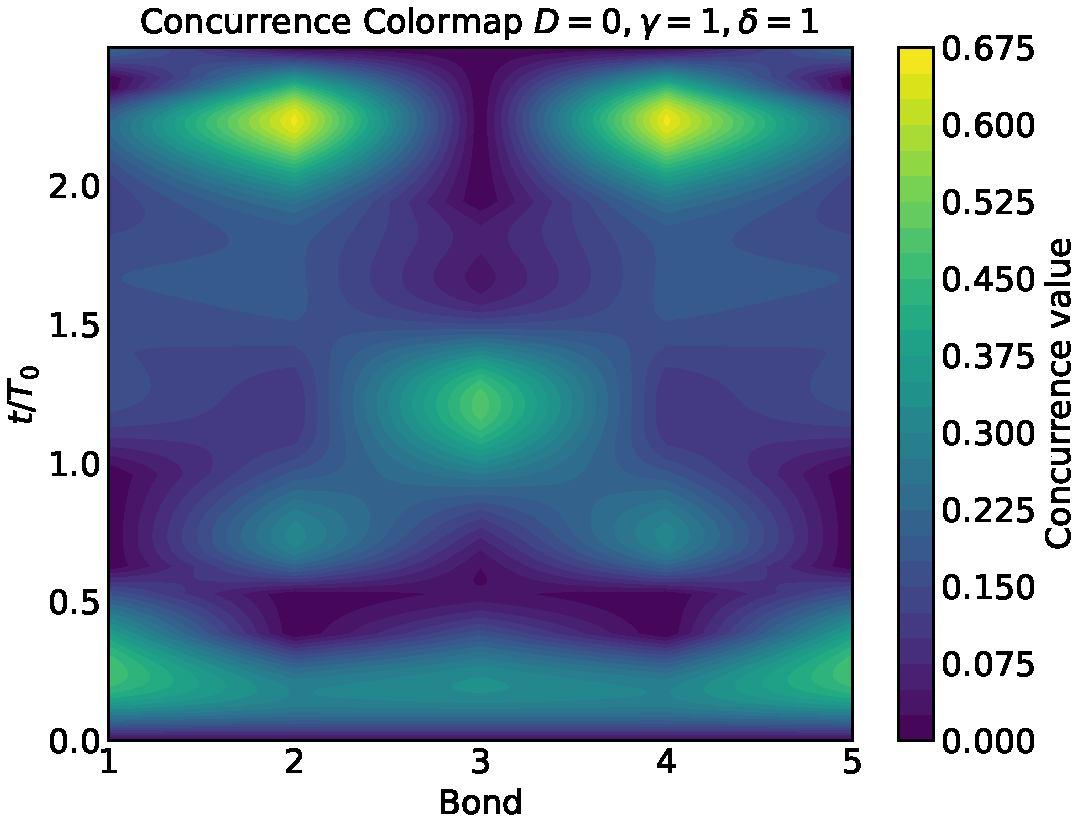
\includegraphics[width=\linewidth]{results_and_discussion/6_qubits/up_down_with_ana_0_1_1.pdf}
        \caption{Concurrence for \( D = 0, \gamma = 1, \delta = 1 \)}
        \label{fig:6q_0_1_1}
    \end{subfigure}

    \vspace{0.5cm}

    \begin{subfigure}[b]{0.48\textwidth}
        \centering
        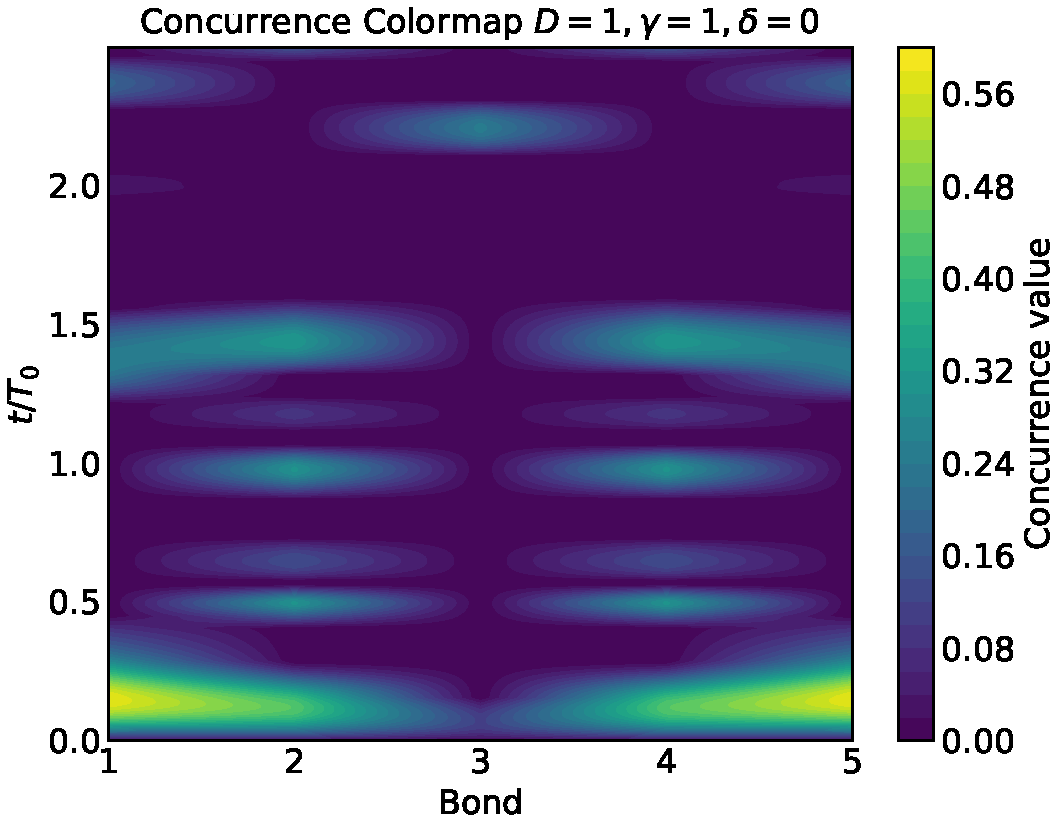
\includegraphics[width=\linewidth]{results_and_discussion/6_qubits/up_down_with_ana_1_1_0.pdf}
        \caption{Concurrence for \( D = 1, \gamma = 1, \delta = 0 \)}
        \label{fig:6q_1_1_0}
    \end{subfigure}
    \hfill
    \begin{subfigure}[b]{0.48\textwidth}
        \centering
        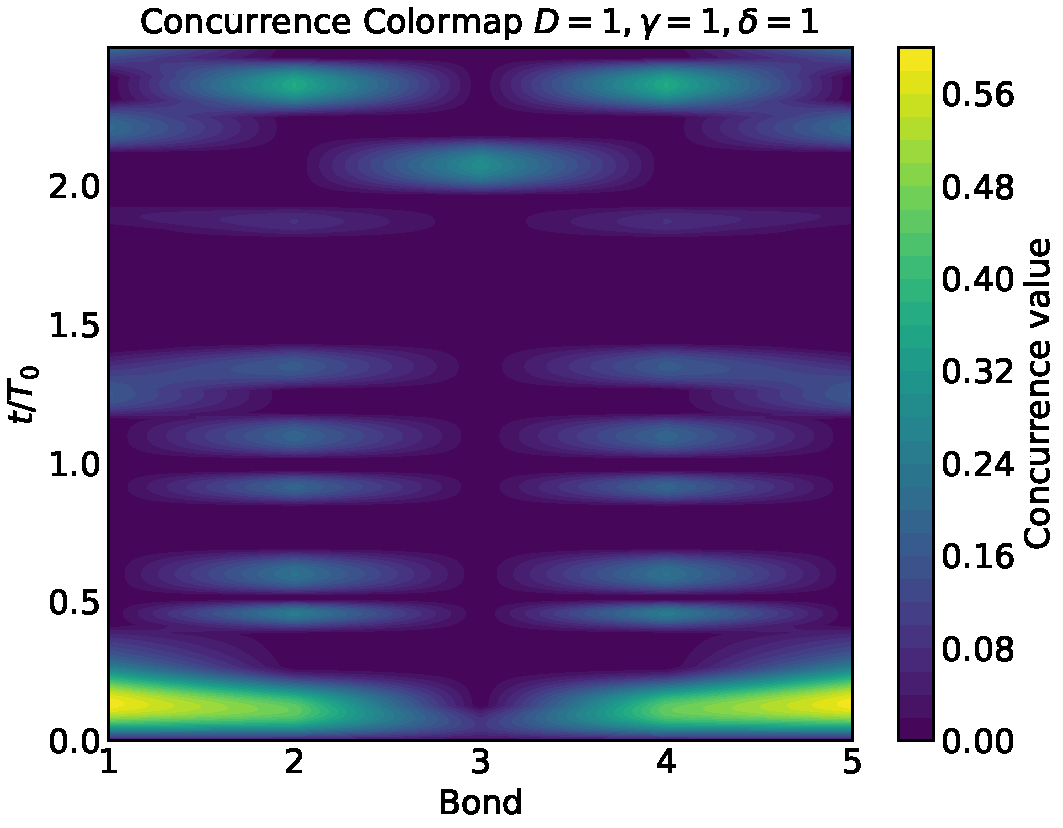
\includegraphics[width=\linewidth]{results_and_discussion/6_qubits/up_down_with_ana_1_1_1.pdf}
        \caption{Concurrence for \( D = 1, \gamma = 1, \delta = 1 \)}
        \label{fig:6q_1_1_1}
    \end{subfigure}

    \caption{Concurrence for different values of \( D \) and \( \delta \) with \( \gamma = 1 \) in a 6-qubit system. The plots illustrate how these parameters affect the entanglement within the system over time.}
    \label{fig:concurrence_comparison_6qubits}
\end{figure}





The results indicate that the Dzyaloshinskii-Moriya interaction (DMI) significantly influences the entanglement properties of the 
system. Specifically, the concurrence values increase when the DMI constant \(D\) is set to 1, implying that the DMI fosters 
stronger entanglement between the qubits in the lattice. This enhancement is evident when comparing cases with \(D = 0\) and 
\(D = 1\), where the latter consistently shows higher concurrence values.

However, the anisotropy parameter \(\delta\) and the correction factor \(\gamma\) introduce competing effects. When 
\(\delta = 1\) and \(\gamma = 1\), the concurrence is lower compared to when \(\delta = 0\) and \(\gamma = 1\), even 
in the presence of DMI. This reduction suggests that the anisotropy, along with \(\gamma\), can counteract the positive 
impact of DMI on entanglement. The interplay between these parameters likely alters the symmetry and interaction strength
within the lattice, thereby influencing the entanglement.

In scenarios where \(D = 0\), the system still exhibits significant entanglement, particularly when 
\(\gamma = 1\) and \(\delta = 0\), with concurrence values reaching up to approximately 0.81. 
This demonstrates that the Heisenberg XY model itself supports strong entanglement, but this can be 
modulated by the presence of DMI and adjustments to \(\delta\) and \(\gamma\).




